% This LaTeX was auto-generated from MATLAB code.
% To make changes, update the MATLAB code and export to LaTeX again.

\documentclass{article}

\usepackage[utf8]{inputenc}
\usepackage[T1]{fontenc}
\usepackage{lmodern}
\usepackage{graphicx}
\usepackage{color}
\usepackage{hyperref}
\usepackage{amsmath}
\usepackage{amsfonts}
\usepackage{epstopdf}
\usepackage[table]{xcolor}
\usepackage{matlab}
\usepackage[paperheight=795pt,paperwidth=614pt,top=72pt,bottom=72pt,right=72pt,left=72pt,heightrounded]{geometry}
%\usepackage[paperheight=11in,paperwidth=8.5in,top=1in,bottom=1in,left=1in,right=1in]{geometry}


\sloppy
\epstopdfsetup{outdir=./}
\graphicspath{ {./Laboratorio_grupal_final_v5_media/} }

\matlabhastoc

\begin{document}

\label{T_85C79F78}
\matlabtitle{Laboratorio: optimización sin restricciones}

\begin{par}
\begin{flushleft}
\textbf{Autores (Grupo 4):} Javier Blanco Álvarez, Pablo Castañeda Fuentes, Lucía Royo Pascual, Ferrán Soto Moscardó, Jesús Gallinal Moreno.
\end{flushleft}
\end{par}

\begin{par}
\begin{flushleft}
\textbf{Asignatura: }Optimización
\end{flushleft}
\end{par}

\matlabtableofcontents{ÍNDICE}

\label{H_4DC2A7BE}
\matlabheading{RESUMEN}

\begin{par}
\begin{flushleft}
En esta práctica se examina la aplicación de métodos de optimización del descenso de gradiente para determinar superficies mínimas de revolución, comparando enfoques de pasos fijos y variables. Se implementaron métodos de Fibonacci y Búsqueda dicotómica para la optimización de pasos, analizando su efectividad para encontrar soluciones óptimas. Partiendo de dos funciones iniciales (una línea recta y una parábola), examinamos el comportamiento de convergencia y la precisión de la solución en diferentes niveles de discretización. Con esta práctica se demuestra la implementación práctica de técnicas de optimización multivariable sin restricciones al tiempo que enfatiza la importancia de la selección adecuada de pasos en problemas de optimización. Los resultados indican la efectividad de los métodos de paso variable para lograr mejores características de convergencia en comparación con los enfoques de paso fijo. 
\end{flushleft}
\end{par}

\begin{par}
\begin{flushleft}
\textbf{Palabras clave:} Optimización sin restricciones, descenso del gradiente, método del trapecio, superficies de revolución, Fibonacci, bñusqueda dicotómica. 
\end{flushleft}
\end{par}


\label{H_6BD9FD3F}
\matlabheading{INTRODUCCIÓN}

\begin{par}
\begin{flushleft}
El estudio de superficies mínimas de revolución mediante la optimización del descenso de gradientes representa una combinación útil y rigurosa entre el cálculo de variaciones y los métodos numéricos. En esta práctica se explora la implementación del descenso de gradiente con tasas de aprendizaje fijas y variables para encontrar la superficie de revolución óptima que minimice el área. El análisis abarca dos condiciones iniciales: una línea recta u(x) = 1 y una parábola u(x) = x²-x+1, logrando una comparación integral de los comportamientos de convergencia. El tamaño de paso variable, determinado por Fibonacci y métodos dicotómicos, busca mantener un enfoque adaptativo para la optimización, mejorando potencialmente las tasas de convergencia y la precisión de la solución. En esta práctica examinamos sistemáticamente la relación entre el número de puntos de discretización (N) y la precisión de la solución final obtenida al tiempo que se incluye un estudio detallado de los perfiles de gradiente bajo tamaños de paso fijos y variables, proporcionando información sobre la dinámica de optimización. y características de convergencia.
\end{flushleft}
\end{par}


\label{H_F371E8E9}
\matlabheading{Descripción del laboratorio}

\label{H_AD83CC91}
\matlabheadingtwo{\textbf{Objetivos}}

\begin{par}
\begin{flushleft}
La idea de este Laboratorio es estudiar un caso de optimización sin restricciones multivariables. Justamente, con la implementación del método del gradiente, se espera aproximar una curva que verifica ciertas condiciones. Esta actividad busca fomentar la exploración, comprensión e implementación del método del descenso del gradiente en un problema exigente desde el punto de vista computacional. Así, se espera que se logre determinar la conexión de este método con lo estudiado para la Actividad 1.
\end{flushleft}
\end{par}

\label{H_FA057F60}
\matlabheadingtwo{\textbf{Planteamiento del Problema}}

\begin{par}
\begin{flushleft}
El objetivo para esta entrega consiste en encontrar la curva que une los puntos $\left(0,\ 1\right)$ y $\left(1,\ 1\right)$, de forma que se minimice el área de la superficie de revolución alrededor del eje. Para ello, se quiere minimizar la integral:
\end{flushleft}
\end{par}

\begin{par}
$$I{\left(u\right)}=\int_0^1 u{\left(x\right)}\sqrt{1+{{\left[u^{\prime } {\left(x\right)}\right]}}^2 }\ dx$$
\end{par}

\begin{par}
\begin{center}
Sujeta a las condiciones:  $u{\left(0\right)}=1=u\left(1\right)$                   
\end{center}
\end{par}

\begin{par}
\begin{flushleft}
En realidad, el área deseada es $2\pi I\left(u\right)$. Sin embargo, el factor $2\pi$ no es relevante y se puede normalizar para facilitar los cálculos.
\end{flushleft}
\end{par}

\label{H_3031C1A8}
\matlabheadingtwo{\textbf{Metodología}}

\begin{par}
\begin{flushleft}
Para resolver este problema, realizaremos una discretización del intervalo $\left\lbrack 0,\ 1\right\rbrack$, de forma que tomaremos   intervalos de la forma: ${\left[\frac{j}{n},\ \frac{j+1}{n}\right]}$, para  $0\le j\le n-1$.
\end{flushleft}
\end{par}

\begin{par}
\begin{flushleft}
 Recordemos que si consideramos una función $f\left(x\right)$, la integración por trapecios nos da la fórmula:
\end{flushleft}
\end{par}

\begin{par}
 $$\int_0^1 f{\left(x\right)}dx\approx \sum_{j=0}^{n-1} \frac{f{\left(x_j \right)}+f\left(x_{j+1} \right)}{2}\cdot \frac{1}{n}=\sum_{j=0}^{n-1} T_j \left(f\left(x\right)\right)$$
\end{par}

\begin{par}
\begin{flushleft}
En nuestro caso, tendremos $f\left(x\right)\ =u{\left(x\right)}\sqrt{1+{{\left[u^{\prime } {\left(x\right)}\right]}}^2 }$ y llamaremos $u_j \ =\ u\left(x_j \right)$. Como estamos aproximando   por una poligonal, podemos considerar que:
\end{flushleft}
\end{par}

\begin{par}
$$u^{\prime } {\left(x_j \right)}\approx \frac{u{\left(x_{j+1} \right)}-u{\left(x_j \right)}}{\frac{1}{n}}=n*\left\lbrack u{\left(x_{j+1} \right)}-u\left(x_j \right)\right\rbrack$$
\end{par}

\begin{par}
\begin{flushleft}
Es decir, aproximamos la derivada por la derecha para el punto inicial y por la izquierda en el punto final. Por lo que la aproximación de la integral será:
\end{flushleft}
\end{par}

\begin{par}
\begin{flushleft}
Así pues, se obtiene la siguiente función, que podemos optimizar usando el método del gradiente:
\end{flushleft}
\end{par}

\begin{par}
\begin{flushleft}

\includegraphics[width=\maxwidth{65.73005519317611em}]{image_0}
\end{flushleft}
\end{par}

\label{H_B4981104}
\matlabheadingtwo{\textbf{Implementación}}

\begin{par}
\begin{flushleft}
Para la implementación, se deben seguir los siguientes pasos:
\end{flushleft}
\end{par}

\begin{par}
\begin{flushleft}
 
\end{flushleft}
\end{par}

\begin{itemize}
\setlength{\itemsep}{-1ex}
   \item{\begin{flushleft} Calcular el gradiente de  F                              \end{flushleft}}
   \item{\begin{flushleft} Calcular la curva óptima para los distintos valores de $n$, teniendo en cuenta que: \end{flushleft}}
\end{itemize}

\begin{par}
$$T_j {\left(u\right)}=\frac{1}{2\left(n+1\right)}\cdot {\left(u_{j+1} +u_j \right)}\sqrt{1+{\left(n+1\right)}^2 {{\left(u_{j+1} -u_j \right)}}^2 }$$
\end{par}

\begin{itemize}
\setlength{\itemsep}{-1ex}
   \item{\begin{flushleft} El gradiente está formado por: \end{flushleft}}
\end{itemize}

\begin{par}
$$\nabla F{\left(u_0 ,u_1 ,\ldots,\ u_n \right)}={{\left[g_0 ,g_1 ,\ldots,g_n \right]}}^T$$
\end{par}

\begin{par}
\begin{flushleft}
Donde:
\end{flushleft}
\end{par}

\begin{par}
\begin{center}
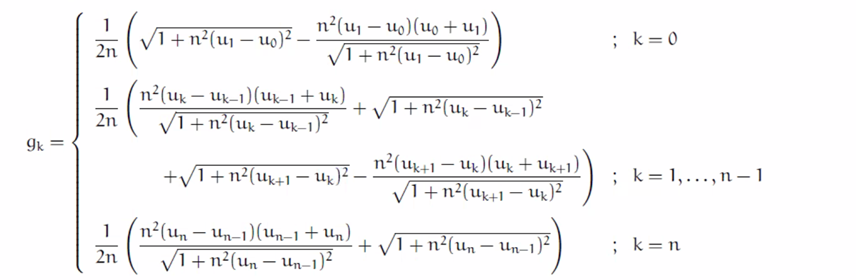
\includegraphics[width=\maxwidth{59.407927747114904em}]{image_1}
\end{center}
\end{par}

\begin{par}
\begin{flushleft}
\textbf{Pautas de elaboración}
\end{flushleft}
\end{par}

\begin{itemize}
\setlength{\itemsep}{-1ex}
   \item{\begin{flushleft} Deberás determinar cuál es la curva tal que, al considerar su sólido de revolución, el área de superficie es mínima. Para hacerlo, ten en cuenta que la incógnita del problema es una función (es necesario discretizarla, como se explica en los apartados anteriores). Al discretizar, el problema se convierte en uno multidimensional de dimensión alta. \end{flushleft}}
   \item{\begin{flushleft} El informe debe entregarse en formato PDF, donde sea posible discriminar cada uno de los aspectos listados en la tabla anexa para la rúbrica. \end{flushleft}}
   \item{\begin{flushleft} Deberás entregar un fichero en \texttt{Matlab} que permita verificar los resultados. Es importante destacar que ese fichero debe correr directamente sin señalar error alguno \end{flushleft}}
\end{itemize}


\label{H_286FC70A}
\matlabheading{Solución Exacta}

\begin{matlabcode}
clear all; close all;

% Valores iniciales asumidos
a0 = 1;
b0 = 0;

% Definimos sistema de ecuaciones para hacer una resolución numérica (más eficiente) 
fun = @(x) [x(1)*cosh(-x(2)/x(1)) - 1;
            x(1)*cosh((1-x(2))/x(1)) - 1];

% Usamos fsolve para solución numérica
options = optimoptions('fsolve', 'Display', 'off');
sol = fsolve(fun, [a0; b0], options);

% Soluciones de a y b
a_val = sol(1);
b_val = sol(2);
fprintf('a = %f\nb = %f\n', a_val, b_val);
\end{matlabcode}
\begin{matlaboutput}
a = 0.848338
b = 0.500000
\end{matlaboutput}
\begin{matlabcode}

% Función para graficar
u_func = @(x) a_val * cosh((x - b_val)/a_val);

% 2D Plot
figure(1)
x_range = 0:0.01:1;
plot(x_range, u_func(x_range), 'LineWidth', 2, 'Color', [0.2 0.5 0.8])
grid on
xlabel('x', 'FontSize', 12, 'FontWeight', 'bold')
ylabel('u', 'FontSize', 12, 'FontWeight', 'bold')
title('Perfil de la Catenaria', 'FontSize', 14, 'FontWeight', 'bold')
axis([0 1 0 max(u_func(x_range))])
set(gca, 'FontSize', 10)
box on
grid minor
\end{matlabcode}
\begin{center}
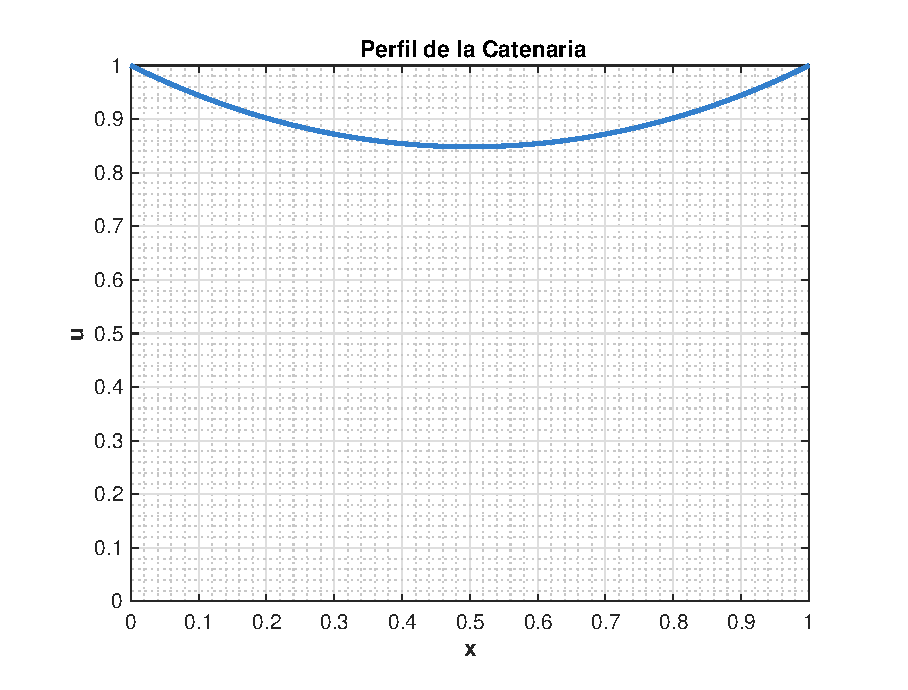
\includegraphics[width=\maxwidth{56.196688409433015em}]{figure_0.eps}
\end{center}
\begin{matlabcode}

% 3D Plot Superficie de revolución
figure(2)
[X,THETA] = meshgrid (x_range, 0:pi/50:2*pi);
R = u_func(X);
Y = R .* cos(THETA);
Z = R .* sin(THETA);

surf(X, Y, Z, 'EdgeColor', 'none', 'FaceAlpha', 0.8)
xlabel('x', 'FontSize', 12, 'FontWeight', 'bold')
ylabel('y', 'FontSize', 12, 'FontWeight', 'bold')
zlabel('z', 'FontSize', 12, 'FontWeight', 'bold')
title('Superficie de revolución Catenaria', 'FontSize', 14, 'FontWeight', 'bold')
axis equal
colormap('parula')  % Parula para mejor contraste
shading interp
lighting gouraud
camlight('headlight')
material([0.7 0.5 0.3 1]) 
grid on
set(gca, 'FontSize', 10)
view(45, 30) 
\end{matlabcode}
\begin{center}
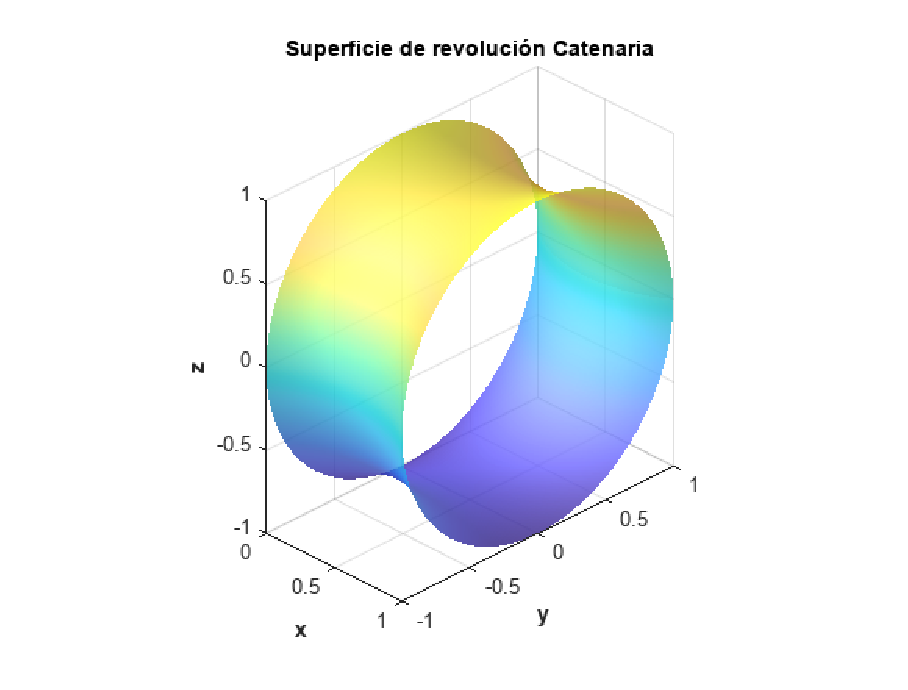
\includegraphics[width=\maxwidth{56.196688409433015em}]{figure_1.eps}
\end{center}
\begin{matlabcode}
    % Derivada de u
    du_dx = @(x) a_val * sinh((x - b_val)/a_val) * (1/a_val);
    % Integrando de la función
    integrando = @(x) 2*pi * u_func(x) .* sqrt(1 + du_dx(x).^2);
    % Integración numérica
    A = integral(integrando, 0, 1);
    
    fprintf('Area de Revolución Exacta = %f\n', A);
\end{matlabcode}
\begin{matlaboutput}
Area de Revolución Exacta = 5.991797
\end{matlaboutput}


\label{H_A57F32C3}
\matlabheading{\textbf{Método de paso fijo}}

\label{H_CE36F4E3}
\matlabheadingtwo{\textbf{Partiendo de recta u(x)  = 1}}

\begin{matlabcode}
clc; clear; close all;
format longg;

% Parámetros
n_vector = [5, 10, 15, 20, 25, 50];
t_vector = [0.001, 0.01, 0.15];

delta_1 = 1e-5;
delta_2 = 0.75;
max_k = 10000;

% Configuraciones de control
verbose = false; % Controla los prints en consola
make_plot = true; % Controla la generación de gráficos

% Estructura para guardar resultados
resultados = struct();

% Crear carpeta para guardar resultados
output_folder = 'resultados_pdf';
if ~exist(output_folder, 'dir')
    mkdir(output_folder);
end

% Salidas
iter = 0;
tic

for n_idx = 1:length(n_vector)
    for t_idx = 1:length(t_vector)
        % Definir parámetros actuales
        n = n_vector(n_idx);
        t = t_vector(t_idx);
        iter = iter + 1;

        % Llamada a la función
        [tabla_iteraciones, u_min_aprox, u_hist, k, texec] = metodo_gradiente_paso_fijo(n, t, delta_1, delta_2, max_k);

        x = 0:1/n:1;
        a = 0.848338;
        u_min_exacta = a * cosh((x - 1/2) / a); % catenaria exacta
        I_min_exacta = (a / 2) * (1 + a * sinh(1 / a)); % Se ha obviado el 2*pi

        F_min_aprox = F(u_min_aprox);

        % Guardar resultados en la estructura
        resultados(iter).n = n;
        resultados(iter).t = t;
        resultados(iter).tabla_iteraciones = tabla_iteraciones;
        resultados(iter).u_min_aprox = u_min_aprox;
        resultados(iter).u_hist = u_hist;
        resultados(iter).k = k;
        resultados(iter).texec = texec;
        resultados(iter).u_min_exacta = u_min_exacta;
        resultados(iter).I_min_exacta = I_min_exacta;
        resultados(iter).F_min_aprox = F_min_aprox;
        resultados(iter).error = abs(F_min_aprox - I_min_exacta);

        % Mostrar resumen en consola si verbose es true
        if verbose
            fprintf('*Solución óptima encontrada en la iteración partiendo de recta u(x)  = 1 %d, para n = %d, t = %f\n\n', k, n, t);
            disp(array2table(tabla_iteraciones(end-3:end, :), 'VariableNames', {'k', 'F(u)', '||u_{k+1} - u_k||', '||grad_F(u_{k+1})||'}));
            fprintf('Valor mínimo de F(u) = F_min_aprox = %f\n|F_min_aprox - I_min_exacta| = %f\n\n', F_min_aprox, abs(F_min_aprox - I_min_exacta));
        end

        % Gráfico controlado por make_plot
        if make_plot
            figure(iter);
            plot(x, u_hist(1:20:end, :)', 'r', ...
                 x, u_min_aprox', 'r', ...
                 x, u_min_exacta, '.-b', 'MarkerSize', 10);
            xlabel('$$x$$', 'Interpreter', 'latex');
            ylabel('$$u(x)$$', 'Interpreter', 'latex');
            legend('$$u_{k}(x)$$', '$$u_{\min}(x)$$', 'Interpreter', 'latex');
            title(['iter = ', num2str(k), ', texec = ', num2str(texec), ' s, n = ', num2str(n), ', t = ', num2str(t)]);
            grid on;

            % Guardar la figura
            saveas(gcf, fullfile(output_folder, sprintf('final_n%d_t%.3f.pdf', n, t)));
        end
    end
end
\end{matlabcode}
\begin{center}
\includegraphics[width=\maxwidth{56.196688409433015em}]{figure_2.eps}
\end{center}
\begin{center}
\includegraphics[width=\maxwidth{56.196688409433015em}]{figure_3.eps}
\end{center}
\begin{center}
\includegraphics[width=\maxwidth{56.196688409433015em}]{figure_4.eps}
\end{center}
\begin{center}
\includegraphics[width=\maxwidth{56.196688409433015em}]{figure_5.eps}
\end{center}
\begin{center}
\includegraphics[width=\maxwidth{56.196688409433015em}]{figure_6.eps}
\end{center}
\begin{center}
\includegraphics[width=\maxwidth{56.196688409433015em}]{figure_7.eps}
\end{center}
\begin{center}
\includegraphics[width=\maxwidth{56.196688409433015em}]{figure_8.eps}
\end{center}
\begin{center}
\includegraphics[width=\maxwidth{56.196688409433015em}]{figure_9.eps}
\end{center}
\begin{matlabcode}

% Mostrar resumen de tiempo total
elapsedTime = toc;
fprintf('El algoritmo tardó %.4f segundos en ejecutarse.\n', elapsedTime);
\end{matlabcode}
\begin{matlaboutput}
El algoritmo tardó 17.5917 segundos en ejecutarse.
\end{matlaboutput}
\begin{matlabcode}

% Mostrar un resumen de la estructura resultados
fprintf('Resumen de resultados:\n');
\end{matlabcode}
\begin{matlaboutput}
Resumen de resultados:
\end{matlaboutput}
\begin{matlabcode}
fprintf('------------------------------------------------------------\n');
\end{matlabcode}
\begin{matlaboutput}
------------------------------------------------------------
\end{matlaboutput}
\begin{matlabcode}
fprintf('| Iteración |     n    |     t     | Iteraciones |  Tiempo(s) |\n');
\end{matlabcode}
\begin{matlaboutput}
| Iteración |     n    |     t     | Iteraciones |  Tiempo(s) |
\end{matlaboutput}
\begin{matlabcode}
fprintf('------------------------------------------------------------\n');
\end{matlabcode}
\begin{matlaboutput}
------------------------------------------------------------
\end{matlaboutput}
\begin{matlabcode}

for i = 1:length(resultados)
    fprintf('|     %2d    |   %3d   | %8.5f |     %4d     |  %8.4f |\n', ...
            i, resultados(i).n, resultados(i).t, resultados(i).k, resultados(i).texec);
end
\end{matlabcode}
\begin{matlaboutput}
|      1    |     5   |  0.00100 |     2641     |    0.1632 |
|      2    |     5   |  0.01000 |      461     |    0.0121 |
|      3    |     5   |  0.15000 |       43     |    0.0008 |
|      4    |    10   |  0.00100 |     4660     |    0.2878 |
|      5    |    10   |  0.01000 |      854     |    0.0216 |
|      6    |    10   |  0.15000 |     10000     |    1.1859 |
|      7    |    15   |  0.00100 |     6480     |    0.7481 |
|      8    |    15   |  0.01000 |     1228     |    0.0417 |
|      9    |    15   |  0.15000 |     10000     |    2.8863 |
|     10    |    20   |  0.00100 |     8167     |    2.9029 |
|     11    |    20   |  0.01000 |     1588     |    0.0802 |
|     12    |    20   |  0.15000 |     10000     |    5.4338 |
|     13    |    25   |  0.00100 |     9756     |    6.7190 |
|     14    |    25   |  0.01000 |     1937     |    0.1407 |
|     15    |    25   |  0.15000 |     10000     |    8.6218 |
|     16    |    50   |  0.00100 |     10000     |   16.4205 |
|     17    |    50   |  0.01000 |     3579     |    1.1634 |
|     18    |    50   |  0.15000 |     10000     |   15.7595 |
\end{matlaboutput}
\begin{matlabcode}
fprintf('------------------------------------------------------------\n');
\end{matlabcode}
\begin{matlaboutput}
------------------------------------------------------------
\end{matlaboutput}
\begin{matlabcode}

% Mostrar detalles de valores mínimos y errores
fprintf('\nDetalles de mínimos y errores:\n');
\end{matlabcode}
\begin{matlaboutput}
Detalles de mínimos y errores:
\end{matlaboutput}
\begin{matlabcode}
fprintf('-------------------------------------------------------------------------\n');
\end{matlabcode}
\begin{matlaboutput}
-------------------------------------------------------------------------
\end{matlaboutput}
\begin{matlabcode}
fprintf('| Iteración | F_min_aprox | I_min_exacta | |F_min_aprox - I_min_exacta| |\n');
\end{matlabcode}
\begin{matlaboutput}
| Iteración | F_min_aprox | I_min_exacta | |F_min_aprox - I_min_exacta| |
\end{matlaboutput}
\begin{matlabcode}
fprintf('-------------------------------------------------------------------------\n');
\end{matlabcode}
\begin{matlaboutput}
-------------------------------------------------------------------------
\end{matlaboutput}
\begin{matlabcode}

for i = 1:length(resultados)
    fprintf('|     %2d    |   %8.5f  |   %8.5f  |        %8.5f         |\n', ...
            i, resultados(i).F_min_aprox, resultados(i).I_min_exacta, resultados(i).error);
end
\end{matlabcode}
\begin{matlaboutput}
|      1    |    0.95563  |    0.95362  |         0.00200         |
|      2    |    0.95558  |    0.95362  |         0.00196         |
|      3    |    0.95558  |    0.95362  |         0.00196         |
|      4    |    0.95420  |    0.95362  |         0.00057         |
|      5    |    0.95412  |    0.95362  |         0.00049         |
|      6    |    1.12904  |    0.95362  |         0.17542         |
|      7    |    0.95397  |    0.95362  |         0.00034         |
|      8    |    0.95384  |    0.95362  |         0.00022         |
|      9    |    1.11507  |    0.95362  |         0.16144         |
|     10    |    0.95391  |    0.95362  |         0.00029         |
|     11    |    0.95375  |    0.95362  |         0.00012         |
|     12    |       -Inf  |    0.95362  |             Inf         |
|     13    |    0.95391  |    0.95362  |         0.00028         |
|     14    |    0.95370  |    0.95362  |         0.00008         |
|     15    |       -Inf  |    0.95362  |             Inf         |
|     16    |    0.95590  |    0.95362  |         0.00228         |
|     17    |    0.95365  |    0.95362  |         0.00002         |
|     18    |       -Inf  |    0.95362  |             Inf         |
\end{matlaboutput}
\begin{matlabcode}
fprintf('-------------------------------------------------------------------------\n');
\end{matlabcode}
\begin{matlaboutput}
-------------------------------------------------------------------------
\end{matlaboutput}
\begin{matlabcode}


% Guardar resultados
save('resultados_t_fijo_recta.mat', 'resultados');


\end{matlabcode}


\label{H_B04DC63F}
\matlabheadingtwo{Partiendo de parábola\textbf{ }u(x) = x\textasciicircum{}2-x+1;}

\begin{matlabcode}
clc; clear; close all;
format longg;

% Parámetros
n_vector = [5, 10, 15, 20, 25, 50];
t_vector = [0.001, 0.01, 0.15];

delta_1 = 1e-5;
delta_2 = 0.75;
max_k = 10000;

% Configuraciones de control
verbose = false; % Controla los prints en consola
make_plot = true; % Controla la generación de gráficos

% Estructura para guardar resultados
resultados = struct();

% Crear carpeta para guardar resultados
output_folder = 'resultados_parabola_pdf';
if ~exist(output_folder, 'dir')
    mkdir(output_folder);
end

% Salidas
iter = 0;
tic

for n_idx = 1:length(n_vector)
    for t_idx = 1:length(t_vector)
        % Definir parámetros actuales
        n = n_vector(n_idx);
        t = t_vector(t_idx);
        iter = iter + 1;

        % Llamada a la función
        [tabla_iteraciones, u_min_aprox, u_hist, k, texec] = metodo_gradiente_paso_fijo_para(n, t, delta_1, delta_2, max_k);

        % Calculo valores exactos
        x = 0:1/n:1;
        a = 0.848338;
        u_min_exacta = a * cosh((x - 1/2) / a); % Catenaria exacta
        I_min_exacta = (a / 2) * (1 + a * sinh(1 / a)); % Se ha obviado el 2*pi

        F_min_aprox = F(u_min_aprox);

        % Guardar resultados en la estructura
        resultados(iter).n = n;
        resultados(iter).t = t;
        resultados(iter).tabla_iteraciones = tabla_iteraciones;
        resultados(iter).u_min_aprox = u_min_aprox;
        resultados(iter).u_hist = u_hist;
        resultados(iter).k = k;
        resultados(iter).texec = texec;
        resultados(iter).u_min_exacta = u_min_exacta;
        resultados(iter).I_min_exacta = I_min_exacta;
        resultados(iter).F_min_aprox = F_min_aprox;
        resultados(iter).error = abs(F_min_aprox - I_min_exacta);

        % Mostrar resumen en consola si verbose es true
        if verbose
            fprintf('* Parabola: Solución óptima encontrada en la iteración %d, para n = %d, t = %f\n\n', k, n, t);
            disp(array2table(tabla_iteraciones(end-3:end, :), 'VariableNames', {'k', 'F(u)', '||u_{k+1} - u_k||', '||grad_F(u_{k+1})||'}));
            fprintf('Valor mínimo de F(u) = F_min_aprox = %f\n|F_min_aprox - I_min_exacta| = %f\n\n', F_min_aprox, abs(F_min_aprox - I_min_exacta));
        end

        % Gráfico controlado por make_plot
        if make_plot
            figure(iter);
            plot(x, u_hist(1:20:end, :)', 'r', ...
                 x, u_min_aprox', 'r', ...
                 x, u_min_exacta, '.-b', 'MarkerSize', 10);
            xlabel('$$x$$', 'Interpreter', 'latex');
            ylabel('$$u(x)$$', 'Interpreter', 'latex');
            legend('$$u_{k}(x)$$', '$$u_{\min}(x)$$', 'Interpreter', 'latex');
            title(['iter = ', num2str(k), ', texec = ', num2str(texec), ' s, n = ', num2str(n), ', t = ', num2str(t)]);
            grid on;

            % Guardar la figura
            saveas(gcf, fullfile(output_folder, sprintf('final_n%d_t%.3f.pdf', n, t)));
        end
    end
end
\end{matlabcode}
\begin{center}
\includegraphics[width=\maxwidth{56.196688409433015em}]{figure_10.eps}
\end{center}
\begin{center}
\includegraphics[width=\maxwidth{56.196688409433015em}]{figure_11.eps}
\end{center}
\begin{center}
\includegraphics[width=\maxwidth{56.196688409433015em}]{figure_12.eps}
\end{center}
\begin{center}
\includegraphics[width=\maxwidth{56.196688409433015em}]{figure_13.eps}
\end{center}
\begin{center}
\includegraphics[width=\maxwidth{56.196688409433015em}]{figure_14.eps}
\end{center}
\begin{center}
\includegraphics[width=\maxwidth{56.196688409433015em}]{figure_15.eps}
\end{center}
\begin{center}
\includegraphics[width=\maxwidth{56.196688409433015em}]{figure_16.eps}
\end{center}
\begin{center}
\includegraphics[width=\maxwidth{56.196688409433015em}]{figure_17.eps}
\end{center}
\begin{matlabcode}

% Mostrar tiempo total de ejecución
elapsedTime = toc;
fprintf('El algoritmo tardó %.4f segundos en ejecutarse.\n', elapsedTime);
\end{matlabcode}
\begin{matlaboutput}
El algoritmo tardó 16.1329 segundos en ejecutarse.
\end{matlaboutput}
\begin{matlabcode}

% Mostrar resumen de resultados
fprintf('\nResumen de resultados:\n');
\end{matlabcode}
\begin{matlaboutput}
Resumen de resultados:
\end{matlaboutput}
\begin{matlabcode}
fprintf('------------------------------------------------------------\n');
\end{matlabcode}
\begin{matlaboutput}
------------------------------------------------------------
\end{matlaboutput}
\begin{matlabcode}
fprintf('| Iteración |     n    |     t     | Iteraciones |  Tiempo(s) |\n');
\end{matlabcode}
\begin{matlaboutput}
| Iteración |     n    |     t     | Iteraciones |  Tiempo(s) |
\end{matlaboutput}
\begin{matlabcode}
fprintf('------------------------------------------------------------\n');
\end{matlabcode}
\begin{matlaboutput}
------------------------------------------------------------
\end{matlaboutput}
\begin{matlabcode}

for i = 1:length(resultados)
    fprintf('|     %2d    |   %3d   | %8.5f |     %4d     |  %8.4f |\n', ...
            i, resultados(i).n, resultados(i).t, resultados(i).k, resultados(i).texec);
end
\end{matlabcode}
\begin{matlaboutput}
|      1    |     5   |  0.00100 |     4213     |    0.1516 |
|      2    |     5   |  0.01000 |      479     |    0.0085 |
|      3    |     5   |  0.15000 |       45     |    0.0005 |
|      4    |    10   |  0.00100 |     9468     |    1.1461 |
|      5    |    10   |  0.01000 |      945     |    0.0220 |
|      6    |    10   |  0.15000 |     10000     |    1.0227 |
|      7    |    15   |  0.00100 |     10000     |    3.4765 |
|      8    |    15   |  0.01000 |     1462     |    0.0481 |
|      9    |    15   |  0.15000 |     10000     |    3.1095 |
|     10    |    20   |  0.00100 |     10000     |    5.3572 |
|     11    |    20   |  0.01000 |     1974     |    0.0827 |
|     12    |    20   |  0.15000 |     10000     |    5.5138 |
|     13    |    25   |  0.00100 |     10000     |    7.3765 |
|     14    |    25   |  0.01000 |     2482     |    0.1264 |
|     15    |    25   |  0.15000 |     10000     |    7.5965 |
|     16    |    50   |  0.00100 |     10000     |   15.3170 |
|     17    |    50   |  0.01000 |     5004     |    3.3017 |
|     18    |    50   |  0.15000 |     10000     |   14.2142 |
\end{matlaboutput}
\begin{matlabcode}
fprintf('------------------------------------------------------------\n');
\end{matlabcode}
\begin{matlaboutput}
------------------------------------------------------------
\end{matlaboutput}
\begin{matlabcode}

% Mostrar detalles de mínimos y errores
fprintf('\nDetalles de mínimos y errores:\n');
\end{matlabcode}
\begin{matlaboutput}
Detalles de mínimos y errores:
\end{matlaboutput}
\begin{matlabcode}
fprintf('-------------------------------------------------------------------------\n');
\end{matlabcode}
\begin{matlaboutput}
-------------------------------------------------------------------------
\end{matlaboutput}
\begin{matlabcode}
fprintf('| Iteración | F_min_aprox | I_min_exacta | |F_min_aprox - I_min_exacta| |\n');
\end{matlabcode}
\begin{matlaboutput}
| Iteración | F_min_aprox | I_min_exacta | |F_min_aprox - I_min_exacta| |
\end{matlaboutput}
\begin{matlabcode}
fprintf('-------------------------------------------------------------------------\n');
\end{matlabcode}
\begin{matlaboutput}
-------------------------------------------------------------------------
\end{matlaboutput}
\begin{matlabcode}

for i = 1:length(resultados)
    fprintf('|     %2d    |   %8.5f  |   %8.5f  |        %8.5f         |\n', ...
            i, resultados(i).F_min_aprox, resultados(i).I_min_exacta, resultados(i).error);
end
\end{matlabcode}
\begin{matlaboutput}
|      1    |    0.95559  |    0.95362  |         0.00196         |
|      2    |    0.95558  |    0.95362  |         0.00196         |
|      3    |    0.95558  |    0.95362  |         0.00196         |
|      4    |    0.95412  |    0.95362  |         0.00049         |
|      5    |    0.95412  |    0.95362  |         0.00049         |
|      6    |    1.14288  |    0.95362  |         0.18925         |
|      7    |    0.95385  |    0.95362  |         0.00023         |
|      8    |    0.95384  |    0.95362  |         0.00022         |
|      9    |    1.10370  |    0.95362  |         0.15008         |
|     10    |    0.95382  |    0.95362  |         0.00020         |
|     11    |    0.95375  |    0.95362  |         0.00012         |
|     12    |       -Inf  |    0.95362  |             Inf         |
|     13    |    0.95394  |    0.95362  |         0.00032         |
|     14    |    0.95370  |    0.95362  |         0.00008         |
|     15    |       -Inf  |    0.95362  |             Inf         |
|     16    |    0.95565  |    0.95362  |         0.00203         |
|     17    |    0.95364  |    0.95362  |         0.00002         |
|     18    |       -Inf  |    0.95362  |             Inf         |
\end{matlaboutput}
\begin{matlabcode}
fprintf('-------------------------------------------------------------------------\n');
\end{matlabcode}
\begin{matlaboutput}
-------------------------------------------------------------------------
\end{matlaboutput}
\begin{matlabcode}

% Guardar resultados
save('resultados_t_fijo_parabola.mat', 'resultados');

\end{matlabcode}

\begin{par}
\begin{flushleft}
Ambos métodos de paso fijo, tanto si se inicia la solución del problema con la parábola x\textasciicircum{}2-x+1 como si se toma la constante igual a 1 como punto de inicio, consiguen converger a la solución esperada. De las gráficas y resultados obtenidos se debe comentar la sensibilidad a los parámetros t y n, es decir, el salto por paso y la discretización que se ha seleccionado para resolver el problema.
\end{flushleft}
\end{par}

\begin{par}
\begin{flushleft}
Las gráficas muestran las iteraciones progresivas, en rojo, converginedo a la solución analítica, en azul. Cuando los parámetros t y n no se eligen de manera a decuada; el resultado es la imposibilidad de converger a la solución buscada. Por otra parte, considerar que tanto si se inicia la ejecución con una curva con valores generalmente mayores que la solución analítica (como para la constante 1) o si se inicia con valores inferiores como en el caso de la parábola, el método de gradiente empleado que minimza la superficie de revolución, dirige la solución a la catenaria anteriormente discutida.
\end{flushleft}
\end{par}

\begin{par}
\begin{flushleft}
De los resultados obtenidos se puede comprobar que las mejores soluciones son obtendias para t=0.01; o en su defecto para t pequeños, esto permite suavizar la obtención de la nueva aproximación de u. Aunque puede incurrir en ralentización del cálculo y aumento del número de iteraciones, parece ser la aproximación más robusta para converger a la solución analítica.
\end{flushleft}
\end{par}


\label{H_9B1B6B67}
\matlabheading{\textbf{Método de paso variable}}

\label{H_36F970D7}
\matlabheadingtwo{Gradiente con paso variable para N = 50}

\begin{matlabcode}
clear, clc, close all;
digits(32)
format shortG
tic;
n = 50;           % número de puntos
max_iter = 10000;   % máximo de iteraciones
tol = 1e-5; % tolerancia máxima
integral_method = 'trapezium';
t_opt_metod = 'dico';
verbose = true;
make_plot = true;
[u_opt, min_area, alpha_opt] = min_rev_surface(n, max_iter, tol,integral_method, t_opt_metod, verbose, make_plot);
\end{matlabcode}
\begin{matlaboutput}
=================================================================
SUPERFICIE MÍNIMA DE REVOLUCIÓN - (DICO)
PROGRESO DE OPTIMIZACIÓN - N = 50 PUNTOS
=================================================================
Iteración    Área            t               Norma Gradiente
-----------------------------------------------------------------
2970         0.937915        0.011960        0.924460       
2980         0.937915        0.011960        0.924559       
2990         0.937915        0.011960        0.924441       
3000         0.937918        0.011967        0.924534       
3010         0.937917        0.011960        0.924829       
3020         0.937917        0.011960        0.924910       
3030         0.937919        0.011967        0.924799       
3040         0.937920        0.011967        0.924909       
3050         0.937919        0.011960        0.925227       
3060         0.937920        0.011967        0.924938       
-----------------------------------------------------------------
\end{matlaboutput}
\begin{center}
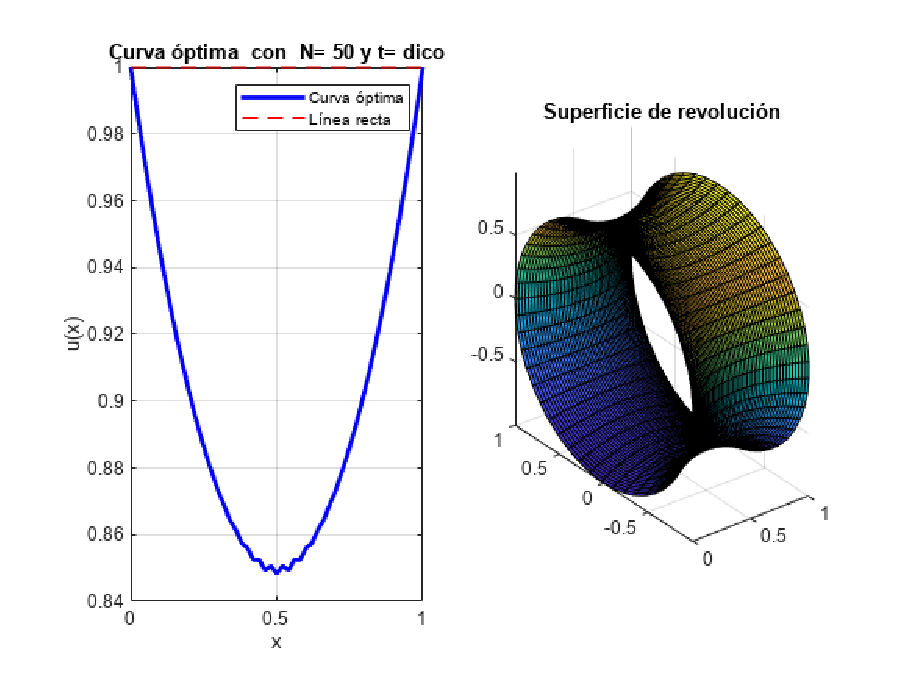
\includegraphics[width=\maxwidth{56.196688409433015em}]{figure_18.eps}
\end{center}
\begin{matlabcode}
elapsedTime = toc;
% Muestra el tiempo transcurrido
fprintf('El algoritmo tardó %.4f segundos en ejecutarse.\n', elapsedTime);
\end{matlabcode}
\begin{matlaboutput}
El algoritmo tardó 0.4047 segundos en ejecutarse.
\end{matlaboutput}


\label{H_A7252E70}
\matlabheadingtwo{Gradiente con paso variable para distintos puntos}

\begin{matlabcode}
clear, clc, close all;
digits(32)
format shortG

% ********************************************************************%
% ******************* BENCHMARK **************************************%
%% Con tolerancia constante y 32 digitos de precisión
tic;
max_iter = 10000;   % máximo de iteraciones
tol = 1e-5; % tolerancia máxima
n_values = [5, 10, 15, 20, 25, 50, 75]; % rectas inexactas no tolera n < 15
integral_methods = {'trapezium'};
t_opt_methods = {'fibo', 'dico'};

results = table('Size', [numel(n_values)*numel(integral_methods)*numel(t_opt_methods), 6], ...
    'VariableTypes', {'double', 'double', 'double', 'double', 'double', 'string'}, ...
    'VariableNames', {'n','iters','min_area', 't_opt', 'mean_norm_grad', 't_opt_method'});

row = 1;
for n = n_values
    for integral_method = integral_methods
        for t_opt_method = t_opt_methods
            [u_opt, iters, min_area, t_opt, mean_error] = min_rev_surface(n, max_iter, tol, integral_method{1}, t_opt_method{1});
            results.n(row) = n;
            results.iters(row) = iters;
            results.min_area(row) = min_area;
            results.t_opt(row) = t_opt;
            results.mean_norm_grad(row) = mean_error;
            results.t_opt_method(row) = string(t_opt_method{1});
            row = row + 1;
        end
    end
end

disp(results)
\end{matlabcode}
\begin{matlaboutput}
    n     iters    min_area      t_opt      mean_norm_grad    t_opt_method
    __    _____    ________    _________    ______________    ____________

     5      69     0.82285       0.13363       0.87646           "fibo"   
     5      85     0.82273       0.13971       0.86777           "dico"   
    10      66     0.88197      0.070554        0.8939           "fibo"   
    10      47      0.8823      0.057209       0.93436           "dico"   
    15     103     0.90423      0.041098       0.92384           "fibo"   
    15     163     0.90423      0.041081       0.92384           "dico"   
    20     505     0.91582      0.030445        0.9249           "fibo"   
    20     553     0.91582      0.030446       0.92507           "dico"   
    25     807     0.92301      0.024345       0.92488           "fibo"   
    25     891     0.92301      0.024312       0.92539           "dico"   
    50    2990     0.93792      0.011969       0.92485           "fibo"   
    50    3061     0.93792      0.011967       0.92519           "dico"   
    75    5884     0.94306     0.0078838       0.92222           "fibo"   
    75    5976     0.94305      0.007916       0.92113           "dico"   
\end{matlaboutput}
\begin{matlabcode}
elapsedTime = toc;
% Muestra el tiempo transcurrido
fprintf('El algoritmo tardó %.4f segundos en ejecutarse.\n', elapsedTime);
\end{matlabcode}
\begin{matlaboutput}
El algoritmo tardó 0.1093 segundos en ejecutarse.
\end{matlaboutput}
\begin{matlabcode}
save('resultados_t_variable.mat', "results")
\end{matlabcode}

\begin{par}
\begin{flushleft}
En este resumen se muestran los dos métodos (fibonacci) y (dicotomica) para un gradiente de paso variable.
\end{flushleft}
\end{par}


\label{H_32DA2901}
\matlabheading{\textbf{Análisis y resultados}}

\label{H_9B8FAD6A}
\matlabheadingtwo{\textbf{Área minima y el número de puntos N}}

\begin{matlabcode}
figure;

% Crear subplots
subplot(1, 2, 1);
hold on;

% Graficar min_area vs n para el método 'fibo'
plot(results.n(strcmp(results.t_opt_method, 'fibo')), ...
     results.min_area(strcmp(results.t_opt_method, 'fibo')), ...
     '-o', 'DisplayName', 'Fibonacci');
xlabel('Número de puntos (n)');
ylabel('Área mínima');
% Leyendas
legend('Location', 'best');
grid on;

subplot(1, 2, 2);
% Graficar min_area vs n para el método 'dico'
plot(results.n(strcmp(results.t_opt_method, 'dico')), ...
     results.min_area(strcmp(results.t_opt_method, 'dico')), ...
     '-s', 'DisplayName', 'Dicotómica');

% Etiquetas y título comunes
sgtitle('Comparación de métodos de optimización'); % Título general
xlabel('Número de puntos (n)');
% Leyendas
legend('Location', 'best');
grid on;

hold off;
\end{matlabcode}
\begin{center}
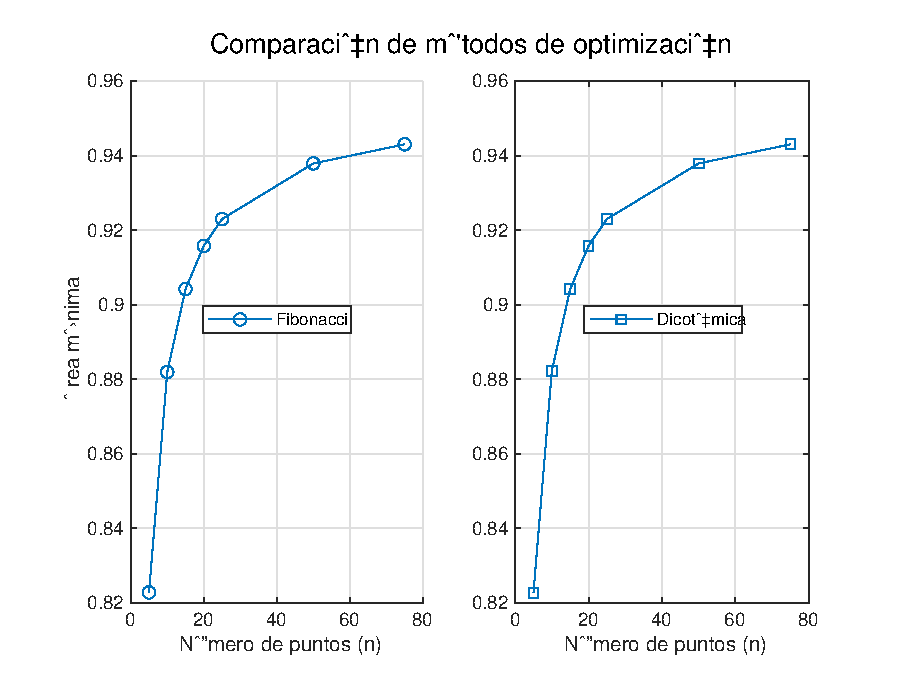
\includegraphics[width=\maxwidth{56.196688409433015em}]{figure_19.eps}
\end{center}

\begin{par}
\begin{flushleft}
Esta figura anterior se muestran dos gráficos que comparan los métodos de optimización de Fibonacci y búsqueda dicotómica. Ambos gráficos muestran un comportamiento de convergencia similar a medida que aumenta el número de puntos (N). El mínimo de superficie se acerca a aproximadamente 0,94 cuando n alcanza los 60 puntos. 
\end{flushleft}
\end{par}

\begin{par}
\begin{flushleft}
Ambos métodos muestran una rápida convergencia inicial hasta aproximadamente n = 20, después de lo cual la mejora se vuelve más gradual. 
\end{flushleft}
\end{par}

\label{H_F7A8891A}
\begin{par}
\begin{flushleft}
El método dicotómico parece tener un comportamiento de progresión ligeramente más suave en comparación con el método de Fibonacci.
\end{flushleft}
\end{par}

\label{H_9859D92F}
\vspace{1em}

\label{H_6EB2E0AD}
\matlabheadingtwo{Cáculo del Área mínima y el método de búsqueda de t óptimo}

\begin{matlabcode}
% Valores únicos
n_values = unique(results.n);
t_opt_methods = unique(results.t_opt_method);

% Preasignación de matriz con n y método de t óptimo
min_area_matrix = zeros(length(n_values), length(t_opt_methods));

% Rellenar la matriz con datos min_area
for i = 1:length(n_values)
    for j = 1:length(t_opt_methods)
        mask = results.n == n_values(i) & results.t_opt_method == t_opt_methods(j);
        min_area_matrix(i, j) = results.min_area(mask);
    end
end

figure;
bar(n_values, min_area_matrix, 'grouped');
xlabel('Número de Puntos (n)');
ylabel('Área Mínima');
title('Área Mínima vs método usado para t óptimo');
legend(t_opt_methods, 'Location', 'best');
grid on;
\end{matlabcode}
\begin{center}
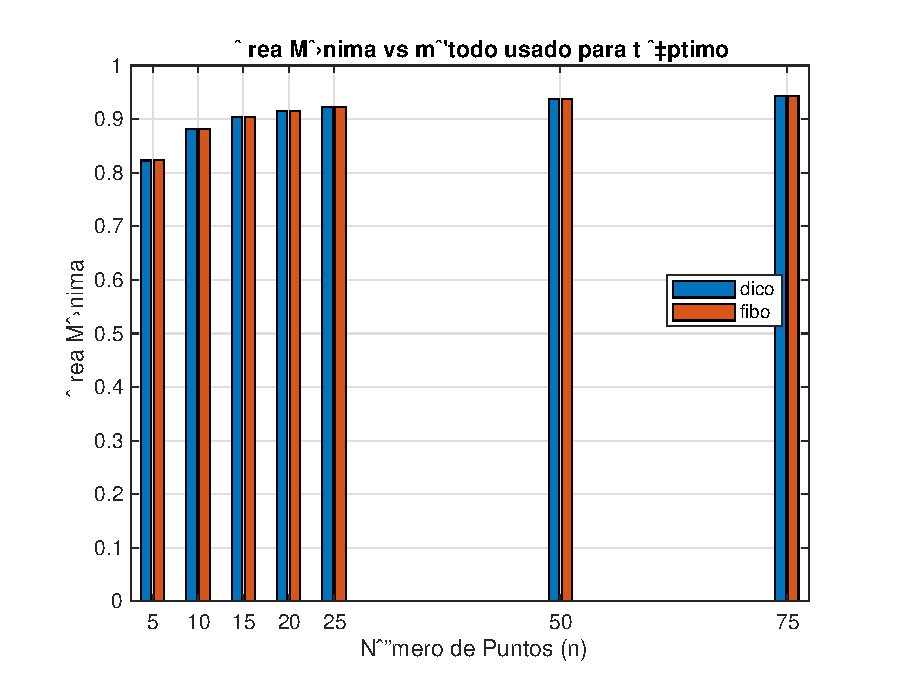
\includegraphics[width=\maxwidth{56.196688409433015em}]{figure_20.eps}
\end{center}
\begin{matlabcode}

\end{matlabcode}

\begin{par}
\begin{flushleft}
En el gráfico de barras se compara el área mínima obtenida por los dos métodos (Búsqueda dicotómica y Fibonacci) a diferentes números de puntos (5, 10, 15, 20, 25 y 50). Los resultados muestran que ambos métodos logran resultados muy similares en todos los valores de puntos y además que el área mínima aumenta con el número de puntos,estabilizándose alrededor de 0,93-0,94
\end{flushleft}
\end{par}

\begin{par}
\begin{flushleft}
No se evidencia una diferencia significativa entre el rendimiento de los dos métodos en términos de área mínima final obtenida.
\end{flushleft}
\end{par}


\label{H_A38AA556}
\matlabheadingtwo{Estudio del perfil del gradiente}

\label{H_C6EA1F5D}
\matlabheadingthree{\textit{Para t fijo}}

\begin{par}
\hfill \break
\end{par}

\begin{matlabcode}
r = load("resultados_t_fijo_recta.mat");

figure;
hold on

n_values = unique([r.resultados.n]);
t_values = unique([r.resultados.t]);

for i = 1:length(n_values)
    current_n = n_values(i);
    idx = find([r.resultados.n] == current_n);
    mean_errors = zeros(size(t_values));
    for j = 1:length(t_values) 
        idx_nt = find([r.resultados.n] == current_n & [r.resultados.t] == t_values(j));

        error_data = r.resultados(idx_nt).tabla_iteraciones(:,4);
        error_data = error_data(error_data < 1);
        if ~isempty(idx_nt)
            mean_errors(j) = mean(error_data);
        end
    end
    
    plot(t_values, mean_errors, ...
         'LineWidth', 1.2, ...
         'DisplayName', sprintf('N = %d', current_n));
end

xlabel('$$t$$', 'Interpreter', 'latex');
ylabel('$$||\nabla(u_{k+1})||$$', 'Interpreter', 'latex');
title('Media Norma Gradiente para t fijo con N puntos');
grid on;
legend('show');

hold off
\end{matlabcode}
\begin{center}
\includegraphics[width=\maxwidth{56.196688409433015em}]{figure_21.eps}
\end{center}
\begin{matlabcode}

\end{matlabcode}

\begin{par}
\begin{flushleft}
Este gráfico muestra la evolución de la norma de gradiente para diferentes números de puntos (Desde 5 hasta 50) en comparación con un paso de tamaño fijo t. Todas las curvas muestran un aumento inicial en la norma del gradiente.Además, los valores de N más bajos (especialmente N = 5) muestran un comportamiento más estable, pero con valores de N más altos muestran disminuciones más notables en la norma del gradiente para distintos valores de t
\end{flushleft}
\end{par}

\begin{par}
\begin{flushleft}
Las curvas divergen considerablemente después de t≈0.05, lo que sugiere que la elección del tamaño del paso se vuelve más crítica con más puntos.
\end{flushleft}
\end{par}

\label{H_96457896}
\matlabheadingthree{Para t variable}

\begin{par}
\hfill \break
\end{par}

\begin{matlabcode}

r_variable = load("resultados_t_variable.mat");
t_opt = r_variable.results.t_opt;
mean_norm_grad = r_variable.results.mean_norm_grad;
n = r_variable.results.n;
t_opt_method = r_variable.results.t_opt_method;

unique_methods = unique(t_opt_method);
shapes = {'o', 's'};
colors = [0.8500 0.3250 0.0980; 0.0000 0.4470 0.7410]; % Paleta mejorada (rojo y azul)

figure;
hold on;

for i = 1:length(unique_methods)
    method_mask = strcmp(t_opt_method, unique_methods{i});
    scatter(t_opt(method_mask), mean_norm_grad(method_mask), 100, ...
        'Marker', shapes{i}, 'MarkerEdgeColor', colors(i, :), ...
        'MarkerFaceColor', colors(i, :), 'DisplayName', unique_methods{i});

    % Añadir etiquetas de n sobre cada punto
    for j = find(method_mask, 4)'
        text(t_opt(j), mean_norm_grad(j) + 0.002, sprintf('%d', n(j)), ...
             'VerticalAlignment', 'bottom', 'HorizontalAlignment', 'center', ...
             'FontSize', 9, 'Color', 'k');
    end
end

% Línea de tendencia por método
for i = 1:length(unique_methods)
    method_mask = strcmp(t_opt_method, unique_methods{i});
    plot(t_opt(method_mask), mean_norm_grad(method_mask), ...
        'Color', colors(i, :), 'LineStyle', '-', 'LineWidth', 1, 'HandleVisibility', 'off');
end

xlabel('$$t_{opt}$$', 'Interpreter', 'latex');
ylabel('$$||\nabla(u_{k+1})||$$', 'Interpreter', 'latex');
title('Media Norma Gradiente vs t opt variable');
legend('Location', 'best');
grid on;
set(gca, 'FontSize', 10);
hold off;
\end{matlabcode}
\begin{center}
\includegraphics[width=\maxwidth{56.196688409433015em}]{figure_22.eps}
\end{center}
\begin{matlabcode}

\end{matlabcode}


\begin{par}
\begin{flushleft}
El gráfico anterior compara los valores t óptimos para los dos métodos, y, de este se desprende que ambos métodos convergen a valores finales similares alrededor de t = 0,15. El método dicotómico (dico) muestra un pico alrededor de t = 0,05. También, el método Fibonacci (fibo) muestra una disminución más gradual. Además, se evidencia que ambos métodos funcionan de manera similar para una mayor cantidad de puntos (50, 25, 15) pero con valores de t pequeños.
\end{flushleft}
\end{par}


\label{H_1444A8A7}
\matlabheading{CONCLUSIONES}

\begin{par}
\begin{flushleft}
La implementación de métodos de descenso de gradiente para encontrar superficies mínimas de revolución demuestra de manera exitosa la aplicación práctica de la optimización multivariada sin restricciones. A través de una exploración sistemática de tamaños de paso fijos y variables, hemos establecido una relación entre los fundamentos teóricos y su implementación computacional. La comparación entre diferentes funciones iniciales y métodos de selección del tamaño de paso proporcionó información valiosa sobre la dinámica de optimización en el ejercicio en cuestión. 
\end{flushleft}
\end{par}

\begin{par}
\begin{flushleft}
Además, esta actividad conecta efectivamente los conceptos introducidos en el tema 2 (búsqueda unidimensional) con desafíos computacionales más complejos, destacando la importancia de una selección de parámetros adecuada y una estrategia de optimización para lograr la convergencia. 
\end{flushleft}
\end{par}

\begin{par}
\begin{flushleft}
La elección del número de puntos (N) tiene un impacto significativo en el comportamiento de optimización, y los valores de N más altos generalmente conducen a soluciones más estables pero más intensivas desde el punto de vista computacional. La selección del tamaño de paso óptimo (t) parece ser más crítica para valores intermedios, mientras que ambos métodos convergen a resultados finales similares.
\end{flushleft}
\end{par}

\begin{par}
\begin{flushleft}
Finalmente, está práctica se centró particularmente en el papel de los tamaños de paso adaptativos en la mejora del rendimiento de la optimización, al tiempo que evidencian los requisitos computacionales inherentes a este tipo de problemas.
\end{flushleft}
\end{par}


\label{H_8A175E69}
\matlabheading{\textbf{REFERENCIAS}}

\begin{itemize}
\setlength{\itemsep}{-1ex}
   \item{\begin{flushleft} Bonnans, J. F., Gilbert, J. C., Lemaréchal, C., \& Sagastizábal, C. A. (2021). Numerical optimization: Theoretical and practical aspects. Springer. \end{flushleft}}
   \item{\begin{flushleft} Boyd, S., \& Vandenberghe, L. (2020). Convex optimization. Cambridge University Press. \end{flushleft}}
   \item{\begin{flushleft} Nocedal, J., \& Wright, S. J. (2022). Numerical optimization (3rd ed.). Springer Science. \end{flushleft}}
   \item{\begin{flushleft} Sun, W., \& Yuan, Y. X. (2021). Optimization theory and methods: Nonlinear programming. Springer. \end{flushleft}}
\end{itemize}

\label{H_7ACC0C35}
\vspace{1em}


\label{H_0EE33824}
\matlabheading{ANEXOS}

\label{H_236C7886}
\matlabheadingtwo{Anexo I: Método Gradiente Paso fijo}

\label{H_37222513}
\matlabheadingthree{Con aproximacióna a una recta u(x)  = 1}

\begin{par}
\hfill \break
\end{par}

\begin{matlabcode}
function [tabla_iteraciones, u, u_hist, k, texec] = metodo_gradiente_paso_fijo(n, t, delta_1, delta_2, max_k)
    k = 0; % índice de iteración
    error_1 = delta_1 + 1; % error ||u_{k+1} - u_k||
    error_2 = delta_2 + 1; % error ||grad_f(u_{k+1})||
    u = ones(n+1, 1); % vector de inicio
    u_hist = u'; % guarda historial de iteraciones
    tabla_iteraciones = [];
    tic;
    while (error_1 > delta_1 || error_2 > delta_2) && k < max_k
    k = k + 1;
    u_nuevo = u - t * grad_F(u);
    u_nuevo(1) = 1; u_nuevo(n+1) = 1; % exijo las condiciones de contorno!!!
    error_1 = norm(u_nuevo - u);
    error_2 = norm(grad_F(u_nuevo));
    tabla_iteraciones = [tabla_iteraciones; k, F(u), error_1, error_2];
    u = u_nuevo;
    u_hist = [u_hist; u'];
    end
    texec = toc;
end

\end{matlabcode}

\label{H_05AC333A}
\matlabheadingthree{Con aproximacióna a una parábola u(x) = x\textasciicircum{}2-x+1;}

\begin{par}
\hfill \break
\end{par}

\begin{matlabcode}
function [tabla_iteraciones, u, u_hist_para, k, texec] = metodo_gradiente_paso_fijo_para(n, t, delta_1, delta_2, max_k)
    k = 0; % índice de iteración
    error_1 = delta_1 + 1; % error ||u_{k+1} - u_k||
    error_2 = delta_2 + 1; % error ||grad_f(u_{k+1})||
    
   
    x_i = 0:1/n:1;
    
    u = ones(n+1,1);% vector de inicio
    for i=2:n
        
        u(i) = x_i(i)^2-x_i(i)+1;
    end
    u_hist_para = u'; % guarda historial de iteraciones
    tabla_iteraciones = [];
    tic;
    while (error_1 > delta_1 || error_2 > delta_2) && k < max_k
    k = k + 1;
    u_nuevo = u - t * grad_F(u);

    u_nuevo(1) = 1; u_nuevo(n+1) = 1; % exijo las condiciones de contorno!!!
    error_1 = norm(u_nuevo - u);
    error_2 = norm(grad_F(u_nuevo));
    tabla_iteraciones = [tabla_iteraciones; k, F(u), error_1, error_2];
    u = u_nuevo;

    u_hist_para = [u_hist_para; u'];
    end
    texec = toc;
end

\end{matlabcode}

\label{H_D6A89215}
\matlabheadingtwo{Anexo II: Función Integral}

\begin{matlabcode}
function integral = F(u)
    n = length(u) - 1;
    integral = 0;
    for j = 1:n
    integral = integral + (u(j+1)+u(j)) * sqrt(1 + (n*(u(j+1)-u(j)))^2);
    end
    integral = integral/(2*n);
end

\end{matlabcode}

\label{H_94D61C00}
\matlabheadingtwo{Anexo III: Función gradiente}

\begin{matlabcode}
function gradiente = grad_F(u)
    l = length(u);
    n = l - 1;
    c = 1/(2*n);
    gradiente(1) = (c - u(1)*n*(u(2)-u(1))) / sqrt(1 + (n*(u(2)-u(1)))^2);
    for j = 2:n
    gradiente(j) = (c + u(j)*n*(u(j)-u(j-1))) / sqrt(1 + (n*(u(j)-u(j-1)))^2) + ...
    (c - u(j)*n*(u(j+1)-u(j))) / sqrt(1 + (n*(u(j+1)-u(j)))^2);
    end
    gradiente(l) = (c + u(l)*n*(u(l)-u(l-1))) / sqrt(1 + (n*(u(l)-u(l-1)))^2);
    gradiente = gradiente';
end


\end{matlabcode}

\label{H_9F04A6B6}
\matlabheadingtwo{Anexo III: Método Gradiente Paso variable}

\begin{matlabcode}
function [u_optimal, n_iter, min_area, alpha_opt, mean_norm_grad] = min_rev_surface(n, max_iter, tol, integral_method, t_opt_method, verbose, make_plot)
    % Marcando parámetros de entrada
    if nargin < 1, n = 100; end        % número de puntos
    if nargin < 2, max_iter = 1000; end % máximo de iteraciones
    if nargin < 3, tol = 1e-4; end % tolerancia por defecto
    if nargin < 4, integral_method = 'trapezium'; end % Método del trapecio por defecto
    if nargin < 5, t_opt_method = 'fibo';  end % método para encontra t óptimo
    if nargin < 6, verbose = false;  end % verbose igual true mostrará las últimas 10 iteraciones
    if nargin < 7, make_plot = false;  end % método para encontra t óptimo

    % Inicialización
    x = linspace(0, 1, n+1);
    u = ones(1, n+1);  % línea recta para y=1
    iter = 0;
    % Se guardan las últimas 10 iteraciones
    last_areas = zeros(1, 10);
    last_alphas = zeros(1, 10);
    last_norms = zeros(1, 10);
    last_iters = zeros(1, 10);

    % Método de optimización sin restricciones (método del gradiente con t variable)
    if strcmp(integral_method, 'trapezium')
        while iter < max_iter
                grad = trapezium_gradient(u, n);

                % establecemos función de línea para búsqueda de alpha
                f = @(alpha) trapezium(u - alpha .* grad, n); 
                df = @(alpha) -sum(grad .* grad); %Sumatoria del vector gradiente  

                % Llamando a la función Fibonacci o Rectas Inexactas para búsqueda de alpha (t) óptimo
                if strcmp(t_opt_method, 'fibo')
                    [alpha, ~] = fibo(f, df, 0, 1, tol);
                elseif strcmp(t_opt_method, 'dico')
                    [alpha, ~] = budi(f, df, 0, 1, tol);
                end
                % Actualizar u a excepción de los puntos u(a) y u(b) que deben ser 1
                u_new = u - alpha .* grad;
                % Criterio de parada
                if iter > 1 && abs(norm(u_new(2:end-1)) - norm(u(2:end-1))) < tol
                    break;
                end

                u(2:end-1) = u_new(2:end-1);
                iter  = iter+1;
                area = trapezium(u, n);

                if mod(iter, 10) == 0
                last_areas = [last_areas(2:end), area];
                last_alphas = [last_alphas(2:end), alpha];
                last_norms = [last_norms(2:end), norm(grad)];
                last_iters = [last_iters(2:end), iter];
                end
        end
        if verbose == true
            fprintf('\n%s\n', '=================================================================');
            fprintf('SUPERFICIE MÍNIMA DE REVOLUCIÓN - (%s)\n', upper(t_opt_method));
            fprintf('PROGRESO DE OPTIMIZACIÓN - N = %d PUNTOS\n', n);
            fprintf('%s\n', '=================================================================');
            fprintf('%-12s %-15s %-15s %-15s\n', 'Iteración', 'Área', 't', 'Norma Gradiente');
            fprintf('%s\n', '-----------------------------------------------------------------');
            
    
            start_idx = find(last_iters > 0, 1);
            if isempty(start_idx), start_idx = 1; end
            
            
            for i = start_idx:10
                if last_iters(i) > 0  % Only print if there was an actual iteration
                    fprintf('%-12d %-15.6f %-15.6f %-15.6f\n', ...
                        last_iters(i), last_areas(i), last_alphas(i), last_norms(i));
                end
            end
            fprintf('%s\n', '-----------------------------------------------------------------');
        end
        u_optimal = u;
        min_area = trapezium(u_optimal, n);
        alpha_opt = alpha;
        mean_norm_grad = mean(norm(grad));
        n_iter = iter;
        % Graficamos
    if make_plot == true
        plot_result(x, u_optimal, t_opt_method);
    end
    end
end
% Gradiente
function grad = trapezium_gradient(u, n)
    grad = zeros(1, n+1);
    grad(1) = (1/(2*n)) * (sqrt(1 + n^2*(u(2) - u(1))^2) - ... 
               (n^2*(u(2) - u(1))*(u(2) + u(1)))/sqrt(1 + n^2*(u(2) - u(1))^2));

    % k = 1,2,...,n-1
    for k = 2:n
        grad(k) = (1/(2*n)) * (sqrt(1 + n^2*(u(k) - u(k-1))^2) + ...
                  (n^2*(u(k) - u(k-1))*(u(k) + u(k-1)))/sqrt(1 + n^2*(u(k) - u(k-1))^2) + ...
                  sqrt(1 + n^2*(u(k+1) - u(k))^2) - ...
                  (n^2*(u(k+1) - u(k))*(u(k+1) + u(k)))/sqrt(1 + n^2*(u(k+1) - u(k))^2));
    end

    % k = n
    grad(n+1) = (1/(2*n)) * (sqrt(1 + n^2*(u(n+1) - u(n))^2) + ... 
                (n^2*(u(n+1) - u(n))*(u(n+1) + u(n)))/sqrt(1 + n^2*(u(n+1) - u(n))^2));
end

% Área bajo la curva método del trapezio
function area = trapezium(u, n)
    area = 0;
    for j = 1:n
        Tj = (u(j) + u(j+1)) * sqrt(1 + (n+1)^2 * (u(j+1) - u(j))^2) / (2*(n+1));
        area = area + Tj;
    end
end

function plot_result(x, u, t_opt_method)
    figure;
    subplot(1,2,1)
    plot(x, u, 'b-', 'LineWidth', 2);
    hold on;
    plot([0,1], [1,1], 'r--');  % Línea recta original
    grid on;
    title(['Curva óptima  con  N= ' num2str(length(x) - 1) ' y t= ' t_opt_method]); 
    xlabel('x');
    ylabel('u(x)');
    legend('Curva óptima', 'Línea recta');
    % Graficar superficie de revolución
    subplot(1,2,2)
    theta = linspace(0, 2*pi, 50);
    [X, T] = meshgrid(x, theta);
    U = repmat(u, length(theta), 1);
    Y = U .* cos(T);
    Z = U .* sin(T);
    surf(X, Y, Z);
    title('Superficie de revolución');
    axis equal;
    grid on;

end

\end{matlabcode}

\label{H_FADDB86F}
\matlabheadingtwo{Anexo IV: Métodos de búsqueda para t óptimo}

\label{H_687E35E5}
\matlabheadingthree{Fibonacci}

\begin{par}
\hfill \break
\end{par}

\begin{matlabcode}
function [x_min,f_min,k, prec, lapse] = fibo(fun,dfun,a,b,tol)
    I0 = [a, b];
    % F0 = fun(I0);
    F0 = [fun(I0(1)), fun(I0(2))];
    w1 = I0(2) - I0(1);
    max_iter = 50;
    epsilon = 1e-6;
    
    tic;
    % Fibonacci serie implementation
    F = zeros(max_iter, 1);
    F(1) = 1; F(2) = 1; n = 2;

    while w1 > tol*F(n)
        n = n+1;
        F(n) = F(n-1) + F(n-2);
    
    end

    % Fibonacci search algorithm
    w = w1*(F(n-2)/F(n-1));
    xa = I0(2) - w; 
    xb = I0(1) + w;
    fa = fun(xa); 
    fb = fun(xb);
    k = 0;
    
    for n=2:n-2
        w = w*(F(n-k-1)/F(n-k));
        if fa > fb
            I0(1) = xa; F0(1) = fa; xa = xb; fa = fb; xb = xa + w; fb = fun(xb);
        else
            I0(2) = xb; F0(2) = fb; xb = xa; fb = fa; xa = xb - w; fa = fun(xa); 
        end
    
        width_interval = abs(I0(2) - I0(1));
    
        if width_interval < tol
            break;
        end
    
    end
    x_min = (I0(2) + I0(1))/2;
    f_min = fun(x_min);
    k = n;
    prec = abs(dfun(x_min));
    lapse = toc;
    lapse = vpa(lapse);
end
\end{matlabcode}

\label{H_B69C9587}
\matlabheadingthree{Búsqueda Dicotómica}

\begin{par}
\hfill \break
\end{par}

\begin{matlabcode}
function [x_min,f_min,k_opt,prec, lapse] = budi(fun,dfun, a, b, tol)
epsilon = 1e-6;
max_iter = 50;
k = 0;

tic;
x1 = (a+b)/2;
xa = x1-(epsilon/2);
xb = x1 + (epsilon/2);

while abs(b-a) >= tol && k < max_iter

if fun(xa) <= fun(xb)
    b=xb; a=a;
elseif fun(xa) > fun(xb)
    a=xa; b=b;
end

x1 = (a + b) /2;
xa = x1-(epsilon/2);
xb = x1 + (epsilon/2);
fl = fun(a);
fr=fun(b);

k = k+1;

end
x_min = (a+b)/2;
f_min = fun(x_min);
k_opt = k;
prec = abs(dfun(x_min));
lapse = toc;
lapse = vpa(lapse);
end
\end{matlabcode}

\end{document}
